\documentclass{article}
\usepackage[a4paper, margin=2.5cm]{geometry}
\usepackage{polski, graphicx, float}
\setcounter{secnumdepth}{0}

\begin{document}
\subsection{Dotychczsowa komunikacja}
\subsubsection{Schemat blokowy}
\begin{figure}[H]
    \centering
    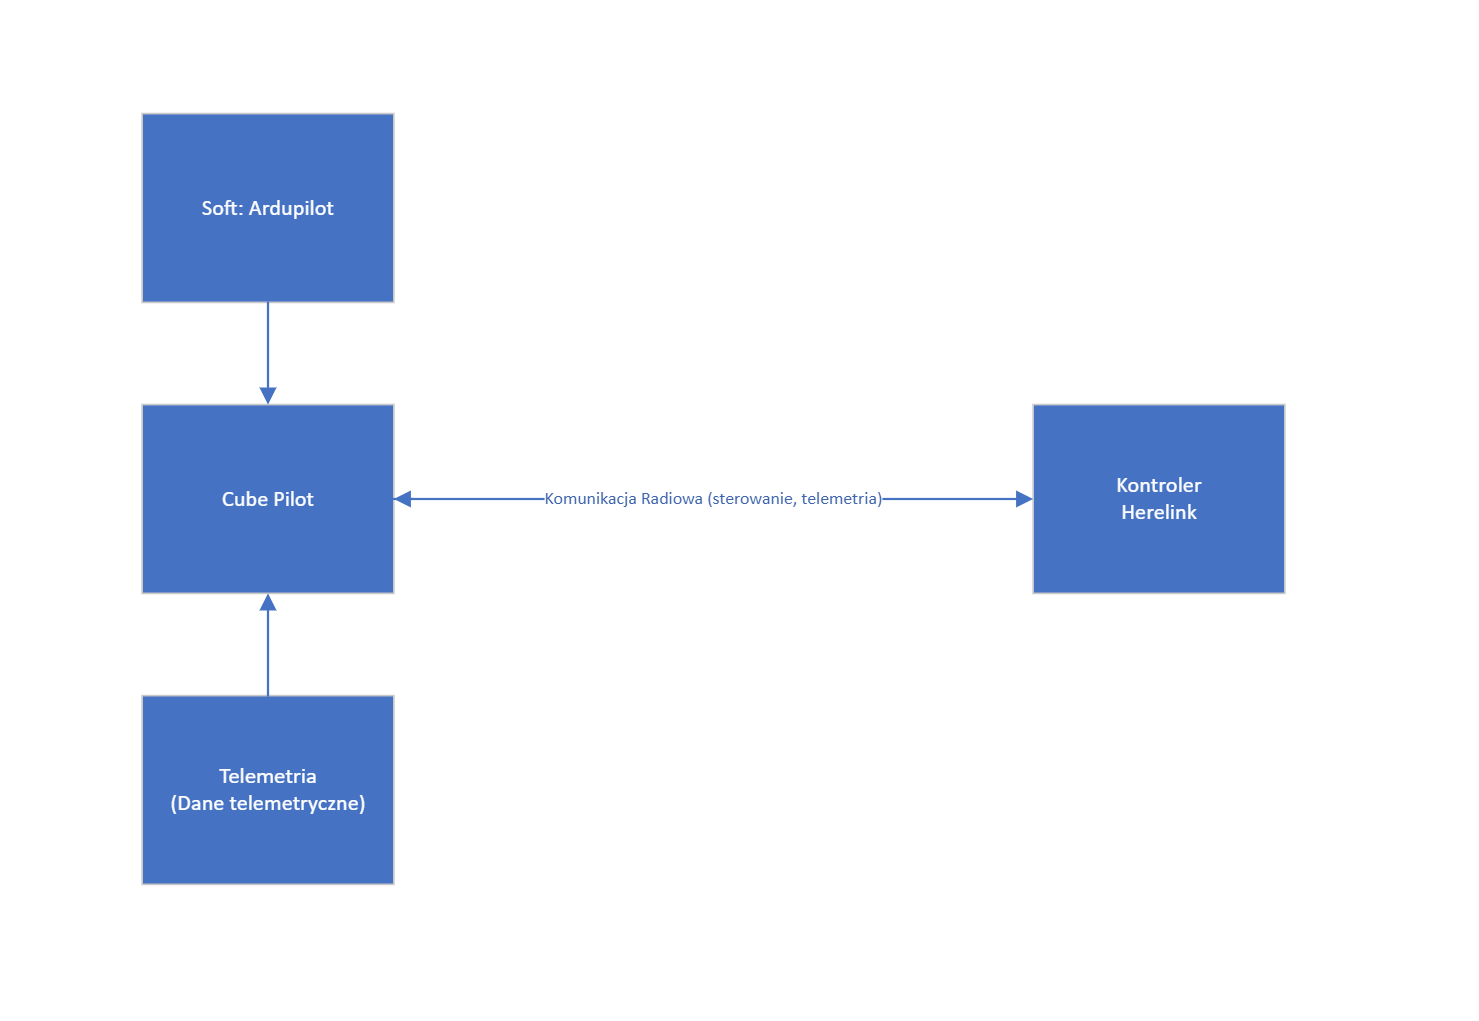
\includegraphics[width=0.7 \textwidth]{przed.png}
    \label{fig:obraz1}
\end{figure}

\subsection{Zmodyfikowana komunikacja po 5G}
\subsubsection{Schemat blokowy}
\begin{figure}[H]
    \centering
    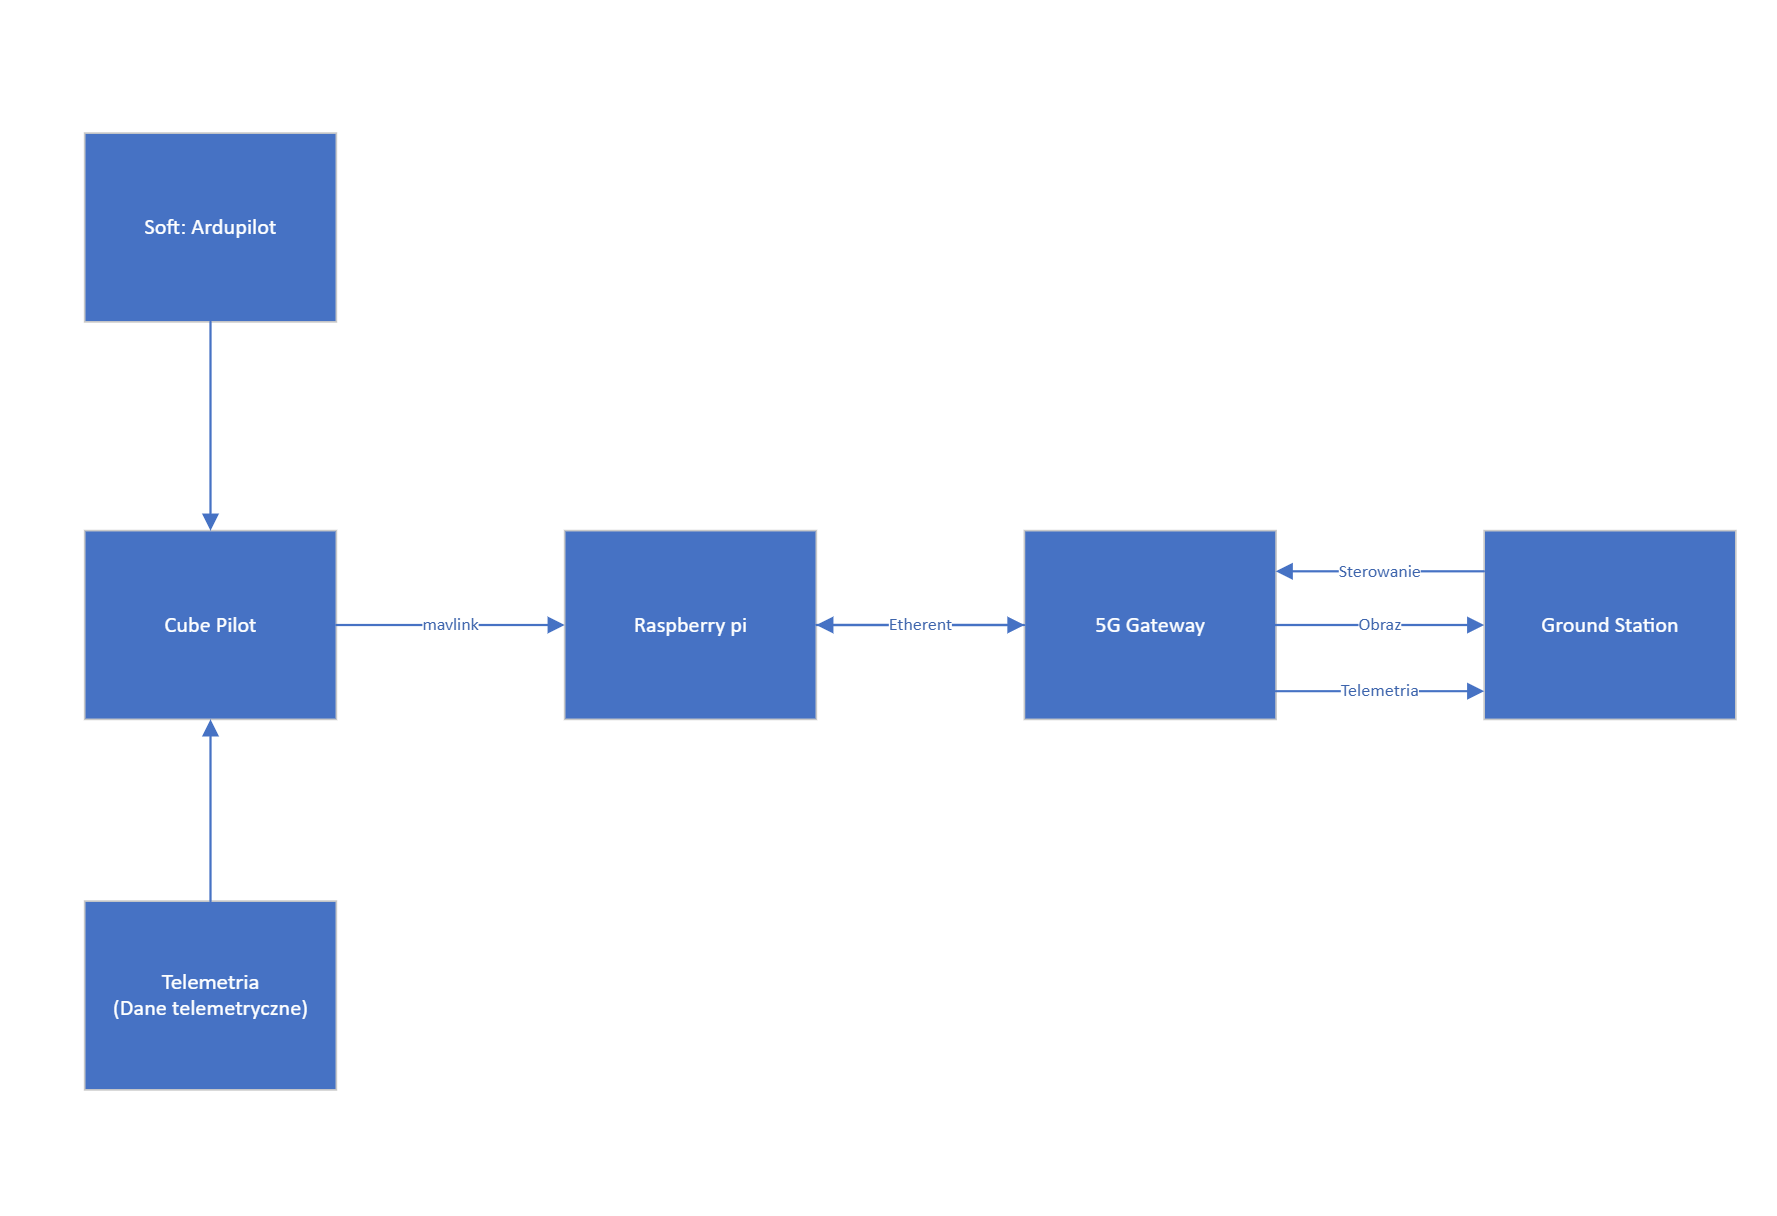
\includegraphics[width=0.7 \textwidth]{po.png}
    \label{fig:obraz2}
\end{figure}

\subsection{Potokoły używane do komunikacji Ardupilota z Ground Station}
\begin{enumerate}
    \item SITL/MAVProxy
    \item UDP
\end{enumerate}

\begin{center}
    Wynika z tego, że do integracji z 5G trzeba użyć protokołu UDP.
\end{center}

\subsection{Źródła}
\begin{enumerate}
    \item https://ardupilot.org/dev/docs/using-sitl-for-ardupilot-testing.html#connecting-other-additional-ground-stations
\end{enumerate}

\end{document}
